\chapter{Implementacija i korisničko sučelje}
		
		
		\section{Korištene tehnologije i alati}
		
		Za izradu web aplikacije korištene su brojne tehnologije koje su pomogle u izradi backend i frontend dijela aplikacije. Razvojna okolina koja se koristila za backend dio je \underline{IDE Eclipse}\footnote{\url{https://www.eclipse.org/}}. Eclipse IDE je programska razvojna okolina pisana u Javi razvijena od tvrtke Eclipse Foundation, a može se koristiti za razvoj aplikacija u raznim programskim jezicima (Java, C, C++, Perl, Python,...). Za izradu backenda koristio se programski jezik \underline{Java}\footnote{\url{https://www.java.com/}} te tehnologije \underline{Java Servleti}\footnote{\url{https://www.oracle.com/technetwork/java/javaee/servlet/index.html}} i \underline{JSP}\footnote{\url{https://www.oracle.com/technetwork/java/}} (Java Servet Pages). Za smještaj servleta korišten je \underline{Apache Tomcat}\footnote{\url{https://tomcat.apache.org/}}. Apache Tomcat je open source Web poslužitelj koji implementira nekoliko Java EE specifikacija kao što su Java Servlet, JSP (Java Servlet Pages), Java EL (Java Expression Language). Može se koristiti kao samostalan web server ili kao poslužitelj za servlete i Java Server Pages (JSP) integriran s nekim drugim web poslužiteljem.
		Kao web poslužitelj koristi se \underline{Windows Server}\footnote{\url{https://www.microsoft.com/en-us/cloud-platform/windows-server}} virtualna mašina podignuta preko servisa \underline{Microsoft Azure}\footnote{\url{https://portal.azure.com/}} na kojemu su instalirani svi servisi koji podupiru rad web aplikacije i baze podataka. Baza podataka pokrenuta je pomoću sustava \underline{PostgreSQL}\footnote{\url{https://www.postgresql.org/}}. 
		
		Mobilna aplikacija je izgrađena u programskom jeziku Java koristeći razvojnu okolinu \underline{Android studio}\footnote{\url{https://developer.android.com/studio/index.html}}. Mobilna aplikacija spaja se na RESTful dio web poslužitelja preko kojeg vrši prijavu u sustav i dohvaćanje podataka. Dizajna Android aplikacije postignut je korištenjem sustava \underline{Adobe XD}\footnote{\url{https://www.adobe.com/products/xd.html}} i \underline{Google Material Design}\footnote{\url{https://www.material.io/}} kao vizualnim jezikom.
		
		 Pomoću alata \underline{Astah Proffesional}\footnote{\url{https://http://astah.net/editions/professional}} nacrtani su UML dijagrami, a kao sustav za upravljanje izvornim kodom korišten je \underline{Git}\footnote{\url{https://git-scm.com/}}. Udaljeni repozitorij projekta je dostupan na web platformi
		\underline{GitLab}\footnote{\url{https://www.gitlab.com/}}. Članovi tima komunicirali su korištenjem aplikacije \underline{Slack}\footnote{\url{https://www.slack.com/}}.
		
		
	\newpage
		\section{Ispitivanje programskog rješenja}
			
			\textbf{\textit{dio 2. revizije}}\\
			
			 \textit{U ovom poglavlju je potrebno opisati provedbu ispitivanja implementiranih funkcionalnosti na razini komponenti i na razini cijelog sustava s prikazom odabranih ispitnih slučajeva. Studenti trebaju ispitati temeljnu funkcionalnost i rubne uvjete..}
	
			
			\subsection{Ispitivanje komponenti}
			\textit{Potrebno je provesti ispitivanje jedinica (engl. unit testing) nad razredima koji implementiraju temeljne funkcionalnosti. Razraditi \textbf{minimalno 6 ispitnih slučajeva} u kojima će se ispitati redovni slučajevi, rubni uvjeti te izazivanje pogreške (engl. exception throwing). Poželjno je stvoriti i ispitni slučaj koji koristi funkcionalnosti koje nisu implementirane. Potrebno je priložiti izvorni kôd svih ispitnih slučajeva te prikaz rezultata izvođenja ispita u razvojnom okruženju (prolaz/pad ispita). }
			
			
			
			\subsection{Ispitivanje sustava}
			
			 \textit{Potrebno je provesti i opisati ispitivanje sustava koristeći radni okvir Selenium\footnote{\url{https://www.seleniumhq.org/}}. Razraditi \textbf{minimalno 4 ispitna slučaja} u kojima će se ispitati redovni slučajevi, rubni uvjeti te poziv funkcionalnosti koja nije implementirana/izaziva pogrešku kako bi se vidjelo na koji način sustav reagira kada nešto nije u potpunosti ostvareno. Ispitni slučaj se treba sastojati od ulaza (npr. korisničko ime i lozinka), očekivanog izlaza ili rezultata, koraka ispitivanja i dobivenog izlaza ili rezultata.\\ }
			 
			 \textit{Izradu ispitnih slučajeva pomoću radnog okvira Selenium moguće je provesti pomoću jednog od sljedeća dva alata:}
			 \begin{itemize}
			 	\item \textit{dodatak za preglednik \textbf{Selenium IDE} - snimanje korisnikovih akcija radi automatskog ponavljanja ispita	}
			 	\item \textit{\textbf{Selenium WebDriver} - podrška za pisanje ispita u jezicima Java, C\#, PHP koristeći posebno programsko sučelje.}
			 \end{itemize}
		 	\textit{Detalji o korištenju alata Selenium bit će prikazani na posebnom predavanju tijekom semestra.}
			
			\eject 
		
		
		\section{Dijagram razmještaja}
			
			Slika prikazuje dijagram razmještaja u sustavu Internet bankarstva. Klijentsko računalo povezuje se s poslužiteljem putem Web preglednika putem http protokola. Android uređaji koriste Android aplikaciju za komunikaciju s poslužiteljem koja se također odvija http protokolom. Poslužiteljsko računalo sastoji se od Web poslužitelja na kojemu se nalazi Web aplikacija i od DB poslužitelja na kojemu se nalazi baza podataka.
			
			\begin{figure}[H]
				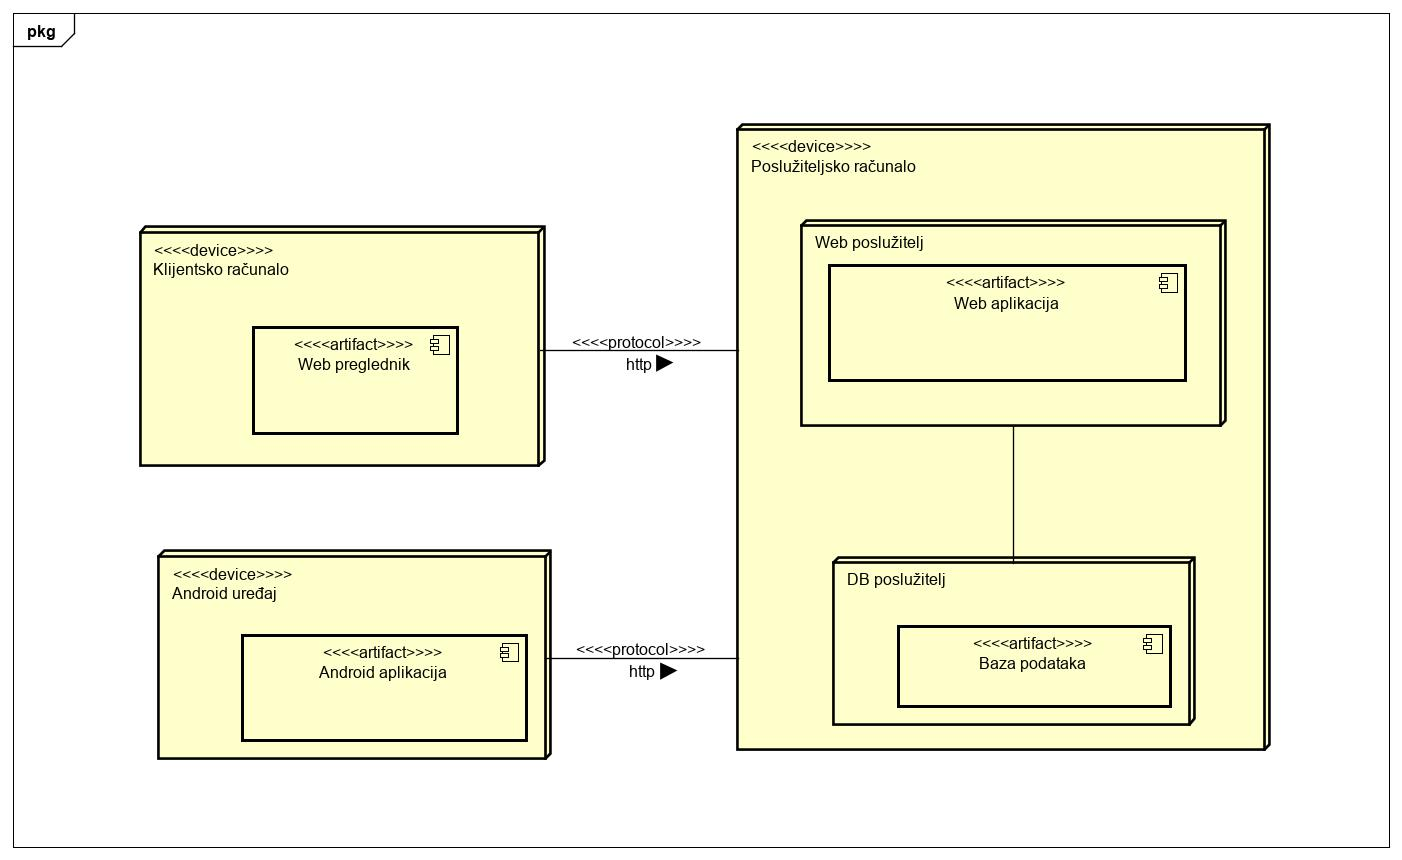
\includegraphics[scale=0.3]{Slike/dijagram_razmjestaja.jpg}
				\centering
				\caption{Dijagram razmještaja}
				\label{fig:dijagram}
			\end{figure}
		
		\section{Upute za puštanje u pogon}
		
		\subsection{Instalacija poslužitelja baze podataka}
		
		Potrebno je preuzeti PostgreSQL (\underline{\url{https://www.postgresql.org/download/}})